% !TEX encoding = UTF-8 Unicode
\documentclass[a4paper]{article}

\usepackage{color}
\usepackage{url}
\usepackage[T2A]{fontenc} % enable Cyrillic fonts
\usepackage[utf8]{inputenc} % make weird characters work
\usepackage{graphicx}
\usepackage{float}
\usepackage[english,serbian]{babel}
\usepackage{tablefootnote}
%\usepackage[english,serbianc]{babel} %ukljuciti babel sa ovim opcijama, umesto gornjim, ukoliko se koristi cirilica

\usepackage[unicode]{hyperref}
\hypersetup{colorlinks,citecolor=green,filecolor=green,linkcolor=blue,urlcolor=blue}

\usepackage{listings}

%\newtheorem{primer}{Пример}[section] %ćirilični primer
\newtheorem{primer}{Primer}[section]

\definecolor{mygreen}{rgb}{0,0.6,0}
\definecolor{mygray}{rgb}{0.5,0.5,0.5}
\definecolor{mymauve}{rgb}{0.58,0,0.82}
\definecolor{blizzardblue}{rgb}{0.67, 0.9, 0.93}

\lstset{ 
  backgroundcolor=\color{white},   % choose the background color; you must add \usepackage{color} or \usepackage{xcolor}; should come as last argument
  basicstyle=\fontsize{10}{1}\ttfamily,        % the size of the fonts that are used for the code
  breakatwhitespace=false,         % sets if automatic breaks should only happen at whitespace
  breaklines=true,                 % sets automatic line breaking
  captionpos=b,                    % sets the caption-position to bottom
  commentstyle=\color{mygreen},    % comment style
  deletekeywords={...},            % if you want to delete keywords from the given language
  escapeinside={\%*}{*)},          % if you want to add LaTeX within your code
  extendedchars=true,              % lets you use non-ASCII characters; for 8-bits encodings only, does not work with UTF-8
  firstnumber=1,                % start line enumeration with line 1000
  frame=single,	                   % adds a frame around the code
  keepspaces=true,                 % keeps spaces in text, useful for keeping indentation of code (possibly needs columns=flexible)
  keywordstyle=\color{blue},       % keyword style
  language=Perl,                 % the language of the code
  morekeywords={*,...},            % if you want to add more keywords to the set
  numbers=left,                    % where to put the line-numbers; possible values are (none, left, right)
  numbersep=5pt,                   % how far the line-numbers are from the code
  numberstyle=\tiny\color{white}, % the style that is used for the line-numbers
  rulecolor=\color{black},         % if not set, the frame-color may be changed on line-breaks within not-black text (e.g. comments (green here))
  showspaces=false,                % show spaces everywhere adding particular underscores; it overrides 'showstringspaces'
  showstringspaces=false,          % underline spaces within strings only
  showtabs=false,                  % show tabs within strings adding particular underscores
  stepnumber=2,                    % the step between two line-numbers. If it's 1, each line will be numbered
  stringstyle=\color{mymauve},     % string literal style
  tabsize=2,	                   % sets default tabsize to 2 spaces
  %title=\lstname                   % show the filename of files included with \lstinputlisting; also try caption instead of title
}

\begin{document}

\title{Perl - smisliti ovde\\ \small{Seminarski rad u okviru kursa\\Metodologija stručnog i naučnog rada\\ Matematički fakultet}}

\author{Aleksandar Vračarević, Jovan Marić,\\ Petar Mićić, Tatjana Radovanović\\ vracarevicaleksandar@gmail.com, maric993@hotmail.com,\\ micicpetar73@gmail.com, tatjana.tasa.95@gmail.com}

%\date{9.~april 2015.}

\maketitle

\abstract{
Cilj ovog rada je da čitaocu, kroz primere koda i pregled glavnih namena programskog jezika Perl, izgradi prvi utisak o jeziku koji je zbog svoje jednostavnosti i čiste sintakse, ali i mnogih mehanizama koji su u njega ugrađeni, uticao na razvoj mnogih jezika. U ovom radu biće prikazano kako se Perl razvijao kroz istoriju, kao i zašto se mnogi programeri opredeljuju za njega.}
\setcounter{tocdepth}{1}
\tableofcontents

\newpage

\section{Uvod}
\label{sec:uvod}

Ve\'cina programskih jezika je osmi\v sljena sa ciljem da reši određenu grupu problema, tako je i programski jezik Perl nastao da reši neke česte probleme pri razvoju softvera. Kao takav programski jezik Perl je stekao veliku popularnost i ima širok domen primene. Perl spada u jezike koji se lako uče jer imaju jednostavnu sintaksu nalik na prirodne jezike. Uz podršku velikog broja modula, Perl programi ostvaruju obimnu funkcionalnost uz minimalan skup naredbi. Iako su njegovu popularnost
preoteli moderniji programski jezici, i dalje predstavlja ozbiljno oružje kod veb programiranja.
U ovom radu \'cemo napraviti pregled osnovnih mogućnosti Perl-a, njegovih karakteristika i specifičnosti. Navešćemo popularna okruženja koja Perl koristi i uputstvo za instalaciju.




\section{Nastanak i razvoj}

Priču o Perlu ne možemo a da ne započnemo sa njegovim stvaraocem Lerijem Volom (eng.~{\em Larry Wall}). Kako sam naglašava u tom trenutku postoje i druga rešenja ali nijedno od njih ne rešava ovu vrstu problema na lak i intuitivan način. Zbog prirode problema nameće se jezik koji će pripadati skript paradigmi. Želeo je da naziv bude kratka reč pozitivne konotacije. Opredeljuje se za pearl(srb.~{\em biser}) ali izostavlja slovo a zbog mogućeg podudaranja sa drugim jezikom u izradi.(Larry Wall, the Guru of Perl, Linux Journal 1. maj 1999)\\

Perl 1.0 postaje dostupan 18. decembra 1987. godine korisnicima Usneta \footnote{Preteča internta na Unix sistemima za komunikaciju širom sveta}, u sekciji posvećenoj ra\v cunarima. Jedna od ideja vodilja prilikom izrade ovog programa bilo je da, kao i bilo koji drugi jezik, raste i evoluira. Ovakav pristup se ogleda u brojnim izborima koje Vol donosi u fazi projektovanja. Kao primer navodimo da je moguće  dotati nove ključne reči u bilo kom trenutku bez narušavanja starih kodova \cite{id}. Još jedna osobina ljudskih jezika je da nije potrebno poznavanje jezika u celini radi efikasnog korisćenja, \v sto važi i za Perl. Ovakve odluke naravno imaju i svoje posledice na performanse koje su za Vola prihvatljive jer on pre svega pokušava da olakša korišćenje programa njegovim korisnicima.\\

\begin{table}

\centering
\begin{tabular}{|l|l|l|} 
\hline
~~ Verzija~ ~        & ~~ Datum             & ~~~~~~~~~~~~~~ Novine                                                                                                                                 \\ 
\hline
~~~ 2.0              & 05.06.1988           & \begin{tabular}[c]{@{}l@{}}-unapređenje regex funkcija\\-rekurzivne subrutine\\-blokovske promenljive\\-foreach petlja\\-sort operator\end{tabular}  \\ 
\hline
~~ 3.0               & 18.10.1989           & \begin{tabular}[c]{@{}l@{}}-podrška za rad u binarnom\\ zapisu\\-prosleđivanje promenljivih \\referencom\\-nove sistemske funkcije\end{tabular}   \\ 
\hline
~~ 4.0               & 21.03.1991           & \begin{tabular}[c]{@{}l@{}}-otklanjanje manjih bagova\\-objedinjena dokumentacija\tablefootnote{U vidu knjige Programing Perl Randal Schwartz, Larry Wall, 1991}\\\end{tabular}                                                      \\ 
\hline
~~ 5.0               & 18.10.1994           & \begin{tabular}[c]{@{}l@{}}-novi interpretator\\-objekti\\-nove funkcije\end{tabular}                                                                 \\ 
\hline
~ 5.6.0              & 22.03.2000           & \begin{tabular}[c]{@{}l@{}}-podrška za utf-8\\-podrška za 64-bitni sistem\\-nadogradnja threadova\end{tabular}                                        \\ 
\hline
\multicolumn{1}{l}{} & \multicolumn{1}{l}{} & \multicolumn{1}{l}{}                                                                                                                                  \\
\multicolumn{1}{l}{} & \multicolumn{1}{l}{} & \multicolumn{1}{l}{}                                                                                                                                 
\end{tabular}
\caption {Pregled osnovnih doprinosa različitih verzija Perl-a}
\end{table}

%Ostajući dosledan svoje zamisli da Perla stalno napreduje u naredne dve godine pojavljuje se čak dve nove verzije 2.0 i 3.0. Najznacajnije novine su nova podrska za regularne izraze, foreach iterator, mogućnost rekurzivnih metoda, rad sa binarnom reprezentacijom i prosleđivanje referenci na promenljive\cite{patchnotes}.\\
Verzija 4.0 prati izdavanje knjige Programing Perl(Randal Schwartz, Larry Wall, 1991). Ovo izdanje se smatra prvom kompletnom dokumentacijom za Perl. Na svojoj naslovnoj strani ima kamilu koja je postala sinonim za Perl u svetu programiranja\cite{perlOrg}.\\

%18. oktobra 1994. godine objavljen je Perl 5.0. Ovo verzija sa sobom donosi do sad najveće promene uključujući i potpuno novi interpretator. Sredinom devedesetih kao dominantna paradigma nameće se objektna pa nas ne čudi da je jedna od glavnih promena u okviru ovoe verzije dodavanje podrske za rad sa objektima.\\
%Do kraja dvadesetog veka izlazi veliki broj novih verzija ali svakako manjeg obima. Najbitnije promene u ovom periodu nisu vezane za sam jezik već se odnose na pojavljivanje Perla na Windwosu kao i na pravljenje velike online baze modula i kodova CPAN(Comprehensive Perl Archive Network).\\
Početak dvadest prvog veka obeležen je nastavkom evoluiranja Perla koji se prilagođava svim potrebama modernog programiranja. Podrška za mrežno programiranje kao i za implementaciju funkcionalne paradigme samo su neki od primera. Sve popularniji pretrazivac DuckDuckGo većinski je implementiran u Perlu\cite{duck}.
%Nemoguce je ne pomenuti Perl 6.0. Ijako član porodice programa Perl nije nastavak Perla 5 već predstavlja jezik za sebe. Dizajner ove verzije je takođe Vol ali se implementira kao projekat otvorenog koda. Prva stabilna verzija objavljena je 2017 godine \footnote[1]{Iz ovog razloga u ovom radu se primarno bavimo verzijom 5}

\subsection{Mesto u razvojnom stablu i uticaji drugih programskih jezika}



Ako u obzir uzmemo činjenicu šta je osnovna namena ovog progrmskog jezika neće nas iznenaditi da u  Perlu možemo naći uticaj šel skripte(eng. Shell script), AWK, sed alata, kao i programskog jezika C kao glavnog predstavnika proceduralne paradigme tog vremena.\cite{friedl2006mastering}\\

\begin{figure}[H]
\centering
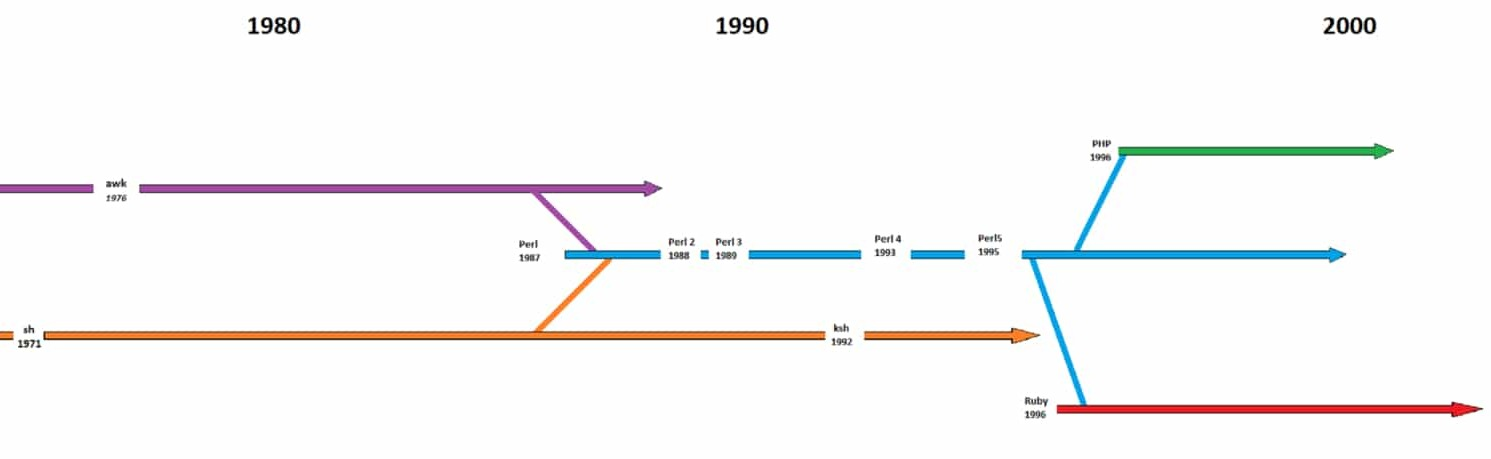
\includegraphics[scale=0.23]{drvorazvoja.jpg}
\caption{Drvo razvoja}
\end{figure}
Iako su počeci Perla mnogo prethodili internetu konstantnim evoluiranjem nikada nije prestao da bude relevantan. Verzija 5.004 donosi nam modul koji obezbeđuje API za pisanje web aplikacija. Krajem devedesetih nazivan je lepkom koji održava internet. Neće nas iznenaditi da u razvojnom stablu programskih jezika zauzima mesto pretka PHP-a.\\
Sredinom poslednje decenije dvadesetog veka Yukihiro Matsumoto želi da objedini moć tekstualnog procesiranja Perla sa Pythonom. Godine 1993. objavljuje programski jezik Ruby.



\section{Osnovna namena, svrhe i mogu\'cnosti}
\label{sec:namena}

Glavna snaga Perla ogleda se u radu sa regularnim izrazima. Tri glavne operacije su uparivanje (eng. matching), zamena uparene niske drugom i prevođenje koje menja karaktere iz liste sa odgovarajućim karakterima iz liste zamena.\cite{id} Postoje brojne modifikacije regex operatora koje olakšavaju korišćenje i pružaju veliki broj opcija programeru. Na usluzi programeru nalaze se i četiri promenljive u kojima se čuvaju rezulatati poslednjeg uparivanja. Imamo pristup sledećim informacijama: da li je došlo do uparivanja, uparenu nisku, nisku pre uparene i nisku posle\cite{friedl2006mastering}. Kada drugi programski jezici predstavljaju svoje mogućnosti vezane za parsiranje teksta i regularne izraze uglavnom to čine poredeći se upravo sa Perlom.\\
Bezbednost je jedna od najznačajnih komponenti svakog programa. Od naglog razvoja mrežnog programiranja bezbednost eksponencijalno dobija na značaju. Već smo pomenuli da Perl pronalazimo kao bekend(eng {\em back end}) skripting jezik u mrežnom programiranju. Veliki razlog za to je tejnted mod rada(eng. {\em Tainted}). Kada Perl operiše u ovom režimu rada svakom podatku koji dolazi od korisnika ili iz okruženja pokretanja, dodaje se malo meta podataka koji ukazuje da ti podaci mogu potencijalno biti problematični. U svakom trenutku u programu se mo\v ze proveriti poreklo podataka i izdvojiti siguran deo istog\cite{modern}.\\
Kao odgovor na sve veću potražnju objektno orijentisanih jezika Perl nudi biblioteku Moose. Moose nudi osnovne mogu\'cnosti kao \v sto su pravljenje klasa, metoda, atributa ali i podržava koncepte kao sto su nasle\dj{}ivanje i preopterećivanje metoda. 

\section{Osnovne osobine}
\label{sec:osobine}

Prvobitna zamisao autora Perl-a, Lerija Vola, bila je da napravi alat koji bi na brz i lak način omogućio napredno rukovanje proizvoljnim tekstualnim datotekama. Jezik je osmišljen sa idejom da se veći značaj prida njegovoj praktičnosti(lakoća korišćenja, efikasnost, kompletnost) nego lepoti(minimalnost, elegancija). Autor smatra da je implementacijom Perla uspeo da izdvoji i iskoristi najbolje funkcionalnosti jezika C, awk, sed i sh\cite{wallperl}.\\
Sintaksa je usko povezana sa sintaksom C-a. Umesto da, kao većina Unix alata, ograničava memoriju, Perl je sposoban da čitav fajl učita kao jednu nisku(ukoliko je dovoljno memorije raspoloživo). Pažljivo osmišljeni mehanizmi poklapanja obrazaca (eng.~{\em pattern matching}) programeru pružaju veoma moćan alat za brzo čitanje velikih datoteka.
Osim za obradu teksta, Perl je tokom godina postao odličan alat za obavljanje raznih sistemskih zadataka, veb programiranje, grafičko programiranje, pristup bazama podataka, mrežno programiranje i mnoge druge zadatke. \\ 

Bitno je još i naglasiti da je Perl interpretirani jezik što omogućava prenosivost jednom napisanih kodova na veliki broj različitih platformi\footnote{Kompletan spisak podržanih platformi može se naći na sledećoj\href{https://perldoc.perl.org/perlport.html#Supported-Platforms}{adresi.}}. Za razliku od strogo (eng.~{\em strictly}) interpretiranih jezika, Perl program se najpre prevodi u sintaksno drvo i nakon toga se izvršava (više reči o korišćenju Perl interpretatora u 
\ref{sec:instalacija}).

\subsection{Tipovi podataka}

Postoji tri tipa ugrađenih podataka: skalari, nizovi skalara i asocijativni nizovi skalara, poznati i kao heševi (eng.~{\em hashes}). Obični nizovi su uređeni i indeksirani brojevima počevši od nule, dok su heševi neuređene kolekcije skalarnih vrednosti indeksirane dodeljenim niskama (ključevima). Skalarne vrednosti mogu biti brojevi, niske i reference uz mogućnost lake i transparentne konverzije između ove tri varijante\footnote{Iako skalar ne može neposredno sadržati više od jedne vrednosti, moguće je dodeliti mu referencu na niz vrednosti.}. Činjenica da Perl dinamički alocira memoriju omogućava pisanje programa otpornih na greške programera poput prekoračenja bafera ili pristupa nedozvoljenoj memoriji. Interpretacija operatora i vrednosti ponekad zavisi od okolnog konteksta. Postoje dva osnovna konteksta: kontekst liste i kontekst skalara.\cite{perldoc}
\begin{primer}
U narednom primeru videćemo da se ista promenljiva može tumačiti na dva različita načina u zavisnosti od konteksta. 
\end{primer}
%TODO: popravi latinicu u okviru komentara
\begin{lstlisting}[label = kontekst]
my @niz = ('Zdravo ', 'svete ', ':D!')    

# @niz se tumaci u kontekstu liste:
# promenljiva @elementi sadrzi kopiju vrednosti promenljive @niz
my @elementi = @niz        

# @niz se tumaci u kontekstu skalara:
# promenljva $broj_elemenata sadrzi broj elemenata promenljive @niz
my $broj_elemenata = @niz
\end{lstlisting} 



\section{Podržane paradigme}

Izjava Lerija Vola da ''Perl nema nikakvu agendu, osim da bude maksimalno korisan maksimalnom broju ljudi.''\cite{walltalk} oslikava težnju Perla da bude što opštiji jezik. Ta tvrdnja je potkrepljena i time što su podržane proceduralna, funkcionalna i objektno-orijentisana paradigma. 

\subsection{Proceduralna paradigma}
%TODO: popraviti drugu referencu
Kao što je već pomenuto u prethodnim poglavljima \ref{sec:namena} i \ref{sec:osobine}, uticaj alata awk, sed i programskog jezika C je primetan u Perlu pa se proceduralni način pisanja programa prirodno nameće. Više primera se može naći u poglavlju \ref{sec:primeri}.

\subsection{Funkcionalna paradigma}

Perl je jezik višeg reda (eng.~{\em higher-order}) koji implementira
koncept dinamičkog pravljenja funkcija i prosleđivanja istih drugim
funkcijama. Dovoljno je moćan da $\lambda$ račun izrazi direktno, u
samom jeziku, bez potrebe za pisanjem posebnog programa za parsiranje
i evaluaciju izraza\cite{Liang:2004:PLC:1060081.1060106,comparing}.
Funkciju sa parametrom x i telom B, $\lambda_x.B$ u Perlu možemo
predstaviti kao \lstinline{sub {my $x = shift; B
\}}. Primena funkcije P na funkciju Q u lambda računu je jednostavno
$(P Q)$, dok je ekvivalentan zapis u Perlu
{\lstinline!$P->($Q)!}.

U sledećem primeru se vidi kako se može napraviti funkcija koja primenjuje prosleđenu funkciju na neki niz element po element.

\begin{lstlisting}[label = mapfun]
sub mapfunkcija{
        my (@rez_lista);
        my ($funkcija, @lista) = @_;
        for (my $i=0;$i<=$#list;$i++)
        {
                $rez_lista[$i] = $funkcija->($lista[$i]);
        }

        return @rez_lista;
};

my @niz = (65, -42, -92);
my $mapme = sub {
        my $x = $_[0];
        return $x + 42;
};

my @rezultat = mapfun ($mapme, @niz);

\end{lstlisting}

Nakon izvršavanja ovog k\^{o}da, u promenljivoj {\lstinline!@rezultat!} se nalaze brojevi 107, 0 i -50. 


\subsection{Objektno-orijentisana paradigma}

Iako Perl nije objektno-orijentisan jezik, može instancirati i manipulisati objektima. Klase su predstavljene paketima, koji moraju posedovati {\lstinline!new!} podrutinu da bi se mogli instancirati. Objekat neke klase se može predstaviti uz pomoć niza ili heša. Enkapsulacija se postiže izdvajanjem interfejsa u pakete. Mehanizam za postizanje polimorfizma je korišćenje ključne reči {\lstinline!bless!}. Ova ključna reč običnu referencu na strukturu podataka označava kao pripadnika nekom paketu i time proširuje mogućnosti te strukture. Nasleđivanje se ostvaruje pomoću specijalnog niza {\lstinline!@ISA!}. Ovaj niz čuva spisak imena modula koji se nasleđuju. U narednom primeru biće prikazani neki od ovih koncepata.\cite{Srinivasan:1997:APP:549810}

\begin{lstlisting}[  label = objPerl]
package Student;    
sub new{            # podrutina za instanciranje klase
    my ($ime, $indeks, $prosek) = @_;
    my $ref_stud = {
        "ime"    =>    $ime,
        "indeks" => $indeks,
        "prosek" => $prosek,
    };
    bless $ref_stud, 'Student'; # objekat se proglasava instancom klase Student
    return $ref_stud;
}

# doseg prethodne klase je ili do kraja datoteke, ili do sledece package kljucne reci

package Profesor;
sub new{            # podrutina za instanciranje klase
    my ($ime, $plata, $fakultet) = @_;
    my $ref_prof = {
        "ime"       =>      $ime,
        "plata      =>    $plata,
        "fakultet"  => $fakultet,
    };
    bless $ref_prof, 'Profesor'; # objekat se proglasava instancom klase Profesor
    return $ref_prof;
}

# instanciranje objekata klase Student i Profesor
$laza_lazic = Student::new('Laza Lazic', 123456, 9.0);
$mika_mikic = Profesor::new('Mika Mikic', 100000, 'Matematicki fakultet');

\end{lstlisting}


\section{Najpoznatija okruženja i njihove karakteristike}

Perl je stekao veliku popularnost u ranim danima veba i često se opisuje kao lepak koji održava internet. Stoga će u ovom poglavlju biti opisana dva okruženja za razvoj veb aplikacija uz dodatak već pomenutog Moose okruženja namenjenog da olakša upotrebu Perla u objektno orijentisanom stilu. 

\subsection{Catalyst}

Catalyst je jedno od najrasprostranjenijih Perl okruženja za razvoj veb aplikacija zasnovano na MVC (eng.~{\em Model View Controller}) arhitekturi. Ovo okruženje pruža nivo apstrakcije nad uobičajenim ciklusom zahteva i odgovora. Zahtevi omogućavaju lako gledanje argumenata nadolazećih upita, POST podataka, otpremanje datoteka i zaglavlja dok odgovori pružaju mogućnost postavljanja zaglavlja i vraćanja izlaza klijentu. 

\subsection{Dancer}

Dancer je okvir za pisanje veb aplikacija veoma intuitivne i izražajne sintakse. Modelovan je po uzoru na Ruby radni okvir, Sinatra. Aplikacije se grade navođenjem HTTP glagola, URL-ova (putanja) i metoda za obradu saobraćaja ka tim konkretnim URL-ovima. 

\begin{lstlisting}[label = dancer]
use Dancer2;
# HTTP glagol GET nakon cega sledi koreni URL '\'
# i na kraju anonimna podrutina koja vraca nisku
get '/' => sub { 
  return 'Zdravo svete!';
};
 
start;

# Ukoliko bi se ovaj primer pokrenuo na racunaru, niska 'Zdravo svete!' bi se odstampala kada se veb pregledac uputi na adresu http://localhost:3000 

\end{lstlisting}

\subsection{Moose}

Iako Perl ima podršku za objektno orijentisanu paradigmu, Moose pokušava da pisanje OO programa učini još lakšim i da programerima pruži jednostavnu deklarativnu sintaksu koja bi eliminisala potrebu za pisanjem konstruktora, destruktora i pristupnih metoda. U pozadini se i dalje dešava nešto slično onome opisanom u \href{sec:osobine}, ali je programer zaštićen od tih detalja implementacije i pruža mu se veći stepen apstrakcije.

\begin{lstlisting}[label = moose]
package Student;
# nakon navodjenja sledece linije, paket postaje klasa
use Moose;
has 'ime' => (
    is => 'rw',     # pristupna funkcija koja moze da cita i upisuje vrednosti u atribut ime
    isa => 'Str',   # naglasavamo da atribut ime moze da prima samo niske
);
has 'neki_atribut' => (...)
# instanciranje objekta
use Student;
my student = Student->new(
    ime => 'mika mikic',
    neki_atribut => 'neka vrednost', ...
);
\end{lstlisting}

\section{Instaliranje i pokretanje}
\label{sec:instalacija}

Da bi se uspešno pokretao perl skript potrebno je imati kompajler\footnote{Strogo govoreći, perl program nije ni kompajler ni interpretator. Naime, perl program se najpre predstavi sintaksnim drvetom koje nakon toga izvršava perlov izvršni sistem\cite{glosar}. Imajući ovu činjenicu u vidu, u nastavku rada će biti korišćen naziv kompajler.}. U ovom poglavlju biće objašnjeno njegovo instaliranje na Linux i Windows operativnim sistemima.

\subsection{Instaliranje na Linux operativnom sistemu}
Da bismo instalirali Perl kompajler na Linux operativnom sistemu potrebno je da u terminalu unesemo komandu {\lstinline!sudo apt-get install perl!}. Od vas će se zatražiti da unesete lozinku. Kada se instalira Perl kompajler u terminalu pokrenite sledeću komandu  {\lstinline !curl -L http://xrl.us/installperlnix | bash!}. Kada sve bude gotovo, da biste se uverili da je instalacija uspešno izvršena ili ako želite da proverite koja je verzija Perl-a instalirana, to možete uraditi komandom {\lstinline!perl -v!}.

\subsection{Pokretanje na Linux operativnom sistemu}
Pokretanje Perl skripta na Linux operativnom sistemu se radi na jednostavan način. Potrebno je otvoriti terminal, a zatim uneti komandu {\lstinline!perl <putanja_do_fajla>!}. Ova komanda će pokrenuti izvršavanje skripta.

\subsection{Instairanje na Windows operativnom sistemu}
Pre instalacije na Windows operativnom sistemu poželjno je  prethodno proveriti da nijedna verzija Perla već nije instalirana. Ako želite da deinstalirate prethodnu verziju idite na  Control Panel - Add/Remove programs. Ako i dalje imate C:\textbackslash Strawberry folder, izbrišite ga ili ga preimenujte. Skinite i instalirajte Padre, the Perl IDE/editor. Strawberry Perl je deo instalacije, ali takođe dobijate i mnoge druge korisne CPAN module. Nakon instalacije, možda ćete morati da restartujete računar. Zatim idite na Start meni/All Programs i pronađite folder sa Perlom. U njemu kliknite na Perl komandnu liniju.  Da biste instalirali module iz CPAN-a u komandnoj liniji ukucajte komandu {\lstinline!cpan App::cpanminus!}. Ukoliko želite da  potvrdite da je instalacija uspešna ukucajte {\lstinline!perl -v!}, ovom komandom, takođe, možete proveriti koja je verzija Perl-a instalirana.

\subsection{Pokretanje na Windowsu}
Ako imamo instaliran Padre, the Perl IDE/editor, komande za pokretanje programa možemo zadati i iz editora. U meniju izaberemo Run, a zatim Run Script, mada možemo da pritisnemo taster F5 i skript \'ce biti pokrenut.
Ako želimo, skript možemo pokrenuti i iz komandne linije tako što ukucamo {\lstinline!perl <putanja_do_fajla>!}.

\section{Primeri koda}
\label{sec:primeri}

Sledeći kod predstavlja primer ispisa Hello world programa. Komentare pišemo iza tarabe. Tekst možemo ispisati tako što ga navedemo iza navodnika ili koristeći funkciju qq.
\begin{lstlisting}[ label=hello]
#Komentar
print "Hello, world!\n";
print qq =Did you say "Hello"?\n=;
\end{lstlisting}

Naredni primer demonstrira program koji računa zbir dva broja. Imena promenljivih počinju znakom \$. U komentarima je dato šta koja print naredba ispisuje.
\begin{lstlisting}[label = zbir]
$a = 5;
$b = 4;
print qq =a \= $a\n=; # a = 5
print qq =b \= $b\n=; # b = 4
$zbir = $a + $b;
print qq=a + b \= $zbir\n=; #a + b = 9
\end{lstlisting}
%TODO: dodati referencu na poglavlje gde se spominju konteksti i izmeniti rečenicu "U ovom slučaju ime niza može počinjati i znakom @ i znakom \$." (Kao što je već pomenuto u ref:poglavlje, ime_niza se može tumačiti u dva različita konteksta u zavisnosti od toga da li je naveden znak @ ili znak $)
Nazivi nizova u Perlu su u formatu @naziv\_niza. Niz se može inicijalizovati tako što elemete navedemo u zagradama, razdvojene zarezom. Ako želimo da ispišemo sve elemete niza, to možemo učiniti samo navođenjem imena niza. Određenom članu niza pristupamo tako što njegov indeks navedemo u uglastim zagradama iza naziva niza. U ovom slučaju ime niza može počinjati i znakom @ i znakom \$. Indeks poslednjeg člana niza dobijamo tako što ispred imena niza stavimo \$\#.
\begin{lstlisting}[label=niz]
@dan = ("Danas", "je", "lep", "dan"); 
$broj_reci = @dan; #Broje elementa niza
print "broj reci u recenici \"@dan\" je $broj_reci.\n";
print "@dan[2], $dan[3]\n";
print "Indeks posednjeg elementa je $#dan\n";
\end{lstlisting}
Grananje u programu možemo izvršiti koristeći if-else naredbu. Naredni program prvo učitava broj sa standardnog ulaza, za zatim proverava da li je pozitivan ili je negativan. Uslov se navodi u zagradi, a if i else blok se navode između vitičastih zagrada.
\begin{lstlisting}[  label=ifelse]
$broj = <STDIN>;
if($broj >= 0){
    print "Broj je pozitivan\n";
}
else{
    print "Broj je negativan\n";
}
\end{lstlisting}

Možemo zadavati i argumente komandne linije. Argumentima komandne linije pristupamo isto kao i elementima niza, samo što kao naziv niza navodimo ARGV. Broj argumenata komandne linije možemo dobiti tako što indeks poslednjeg elementa uvećamo za jedan.
\begin{lstlisting}[label=argv]
$br_arg = $#ARGV + 1;
print "Broj argumenata komandne linije je $br_arg: @ARGV\n";
\end{lstlisting}
Sledećim kodom je prikazan primer korišćenja while petlje. Program prihvata argumente sa ulaza i ispisuje ih na ekran. Ključna reč my označava da je domen promenljive samo taj blok. Promenljiva \$in u while petlji nema uticaj na promenljivu sa istim nazivom van petlje.
\begin{lstlisting}[ label=while]
$in = 5;
while(my $in = <>) {
    print $in; #Ispisuje element koji smo uneli
}
print $in; #Ispisuje broj 5
\end{lstlisting}
%Prethodnu petlju mo\v zemo zapisati i na slede\'ci na\v cin.
%\begin{lstlisting}[caption={Unos i ispis elemenata u while petlji}, frame=single, label=while1]
%while(<>) {
%    print;
%}
%\end{lstlisting}
U Perlu možemo koristiti i for petlju na sličan način kao i u programskom jeziku C.
\begin{lstlisting}[label=for]
for(my $i = 0; $i <= $#ARGV; $i++) {
    print "$ARGV[$i]\n";
}
\end{lstlisting}
Funkcije započinju ključnom rečju sub iza koje sledi naziv funkcije. Telo funkcije se piše između vitičastih zagrada. Argumenti se navode u telu funkcije na sledeći način my(lista\_argumenata) = @\_; Poziv funkcije se vr\v si na standardni na\v cin.
\begin{lstlisting}[ label=funkcija]
sub obim_kvadrata {
    my($a) = @_;
    return 4*$a;
}
\end{lstlisting}
%$obim = obim_kvadrata($aa);
%print "$obim\n"; 
%print obim_kvadrata(4);
%print "\n";
%\end{lstlisting}

\begin{primer}
Sledeći kod predstavlja jednostavan način da zamenimo vrednosti dve promenljive.
\begin{lstlisting}[  label=zamena]
$aa = 3;
$bb = 2;
($aa, $bb) = ($bb, $aa);
print "$aa $bb\n";

\end{lstlisting}

\end{primer}

\section{\v Sta je ono što izdvaja Perl?}

Velika Perl Arhiva\cite{cpan} (eng. ~{\em Comprenhensive Perl Archive Network(CPAN)}) 
 predstavlja online skladište Perl programa, dokumentacije i modula koji olakšavaju implementaciju i održavanje Perl projekata. Arhiva čuva oko 180 hiljada modula otvorenog koda napisanih od preko 12 hiljada 
 programera.

Glavni zadatak CPAN-a je da omogu\'ci programerima da prona\dj{}u module koji nisu uklju\v ceni u paket osnovnih modula. Paket osnovnih modula se dobija instalacijom Perl kompajlera. %Neki od njih su 
Modul pod imenom CPAN.pm omogućava lako preuzimanje i instaliranje drugih Perl modula. 


\subsection{Parsiranje tekstualnog sadržaja}
% da je text processing language?, zbog cega je text processing language (sta je to sto omogucava procesiranje teksta), primer koda gde se parsira fajl, onaj primer sa frekvencijom reci u tekstu i da ga objasnim.

Prve verzije Perl programskog jezika su u fokus stavljale obradu i manipulaciju tekstualnog sadržaja. Sama skra\'cenica PERL (Practical Extraction and Reporting Language) prikazuje osnovne namene jezika, a to su izvlačenje nekog sadržaja i generisanje izveštaja na osnovu tog sadržaja.

Naredni primer prikazuje kako na jednostavan način možemo izračunati broj pojavljivanja svake reči u tekstu, pri čemu se za reč smatra niska karaktera koja se sastoji samo od malih i velikih slova abecede.

\begin{lstlisting}[label=simple]
while (my $line = <$fh>) {
   chomp $line;
   foreach my $str (split /^[A-Za-z]+$/, $line) {
       $count{$str}++;
    } 
}
\end{lstlisting}


Dakle, prvo prolazimo kroz fajl (predstavlja referencu na fajl koji smo 
prethodno otvorili) liniju po liniju, zatim iz linije uklanjamo znak za novi red, a potom za svaku reč (smeštenu u promenljivoj \$str) koja odgovara navedenom regularnom izrazu, ažuriramo strukturu u kojoj čuvamo reč i broj izračunatih pojavljivanja. Rezultat rada navedenog 
dela koda je smešten u promenljivoj \$count. \cite{cooksnd}


\subsection{Jednostavno korišćenje regularnih izraza}
% da su reg izrazi "koren" parsiranja nekog teksta, i da perl pruza koriscenje regularnih izraza na elegantan nacin, sta su regularni izrazi, primer koda i da objasnim kod
% da prikazem kako se koriste regularni izrazi u Perl programima na jednostavan nacin.
% da je bogata podrska regularnim izrazima u Perl-u

Važnu ulogu pri manipulaciji tekstualnog sadržaja igraju regularni izrazi. Regularni izrazi su šabloni koji mogu biti prepoznati u nizovima karaktera. Rezultat rada operacije prepoznavanja šablona jeste tačno ili netačno, odnosno da li niz karaktera odgovara datom šablonu ili ne. Perl ima ugradjene mehanizme koji čine rad sa regularnim izrazima lakšim, nalik na alate grep, sed i awk.\cite{sed} %ovde referenca na neki grep sed..., pitati za ovo



Osnovni operatori primene regularnih izraza, koje Perl nudi, jesu $=\sim$ i $!\sim$. U izrazu \$str $=\sim$ m/regex/ se proverava da li se data niska \$str podudara sa regularnim izrazom regex. Regularni izrazi se navode izme\dj{}u dve kose crte. U slučaju da je došlo do poklapanja, izraz vraća 1, a nula inače. Operator $!\sim$ radi suprotno, u slučaju podudaranja vraća 0, a 1 inače.

Postoje tri osnovne operacije sa regularnim izrazima:

\begin{itemize}
  \item Provera podudaranja - m/regex/
  \item Zamena re\v ci - s/regex/word/
  \item Translacija - tr/regex/word/
\end{itemize}

Zamena reči funkcioniše tako što se sva podudaranja regularnog izraza u nisci zamene navedenom niskom. Na primer u izrazu "Volim mačke!" =~ s/mačke/pse, deo niske mačke \' ce biti zamenjen sa pse, i novodobijena niska predstavlja rezultat izraza.

Translacija je slična zameni reči, sa tim što ne koristi regularne izraze prilikom pretrage niske.


\section{Zaključak}
\label{sec:zakljucak}

Ovaj rad prikazuje osnovne osobine programskog jezika Perl, nastanak, istorijski značaj i njegov uticaj. Upoznaje \v citaoca sa sintaksom, glavnim elementima, nekim od naj\v ce\v s\'cih okru\v zenja koje on koristi kao i osnovnim paradigmama koje on podržava. Ono što čini ovaj jezik nezamenljivim oružjem kada je u pitanju tekstualna analiza, jeste ugrađen skup bogatih mehanizama za rad sa regularnim izrazima koji ubrzavaju i olakšavaju razvoj softvera. Oblasti u kojima je Perl pogodan izbor su tako\dj{}e i mrežno programiranje, programiranje baza podataka, veb programiranje i grafičko programiranje. 


\addcontentsline{toc}{section}{Literatura}
\appendix
\bibliography{seminarski} 
\bibliographystyle{plain}


\end{document}

